
\documentclass[]{svmono}

\usepackage{fancybox}
\usepackage{graphicx}
\usepackage{pdfpages}
\usepackage{color}
\usepackage{epstopdf}
\usepackage{geometry}
\usepackage{amsmath}
\usepackage{float}
\usepackage{listings}
\usepackage{verbatim}
\usepackage{booktabs}
\usepackage{tabularx}
\usepackage{longtable}
\usepackage{amsmath}
\usepackage{caption}
\usepackage{wrapfig}

\geometry{
 a4paper,
 total={210mm,297mm},
 left=20mm,
 right=20mm,
 top=20mm,
 bottom=15mm,
 }


\usepackage{subcaption}


\usepackage{enumerate}

\usepackage{bashful}

\usepackage{multicol}


\usepackage{textcomp}
\usepackage{hyperref}
%\usepackage[hyphenbreaks]{breakurl}
%\usepackage[hyphens]{url}


\sloppy
\definecolor{lightgray}{gray}{0.5}
\setlength{\parindent}{20pt}


\definecolor{mygreen}{rgb}{0,0.6,0}
\definecolor{mygray}{rgb}{0.5,0.5,0.5}
\definecolor{mymauve}{rgb}{0.58,0,0.82}

\lstset{ %
  backgroundcolor=\color{white},   % choose the background color; you must add \usepackage{color} or \usepackage{xcolor}
  basicstyle=\footnotesize,        % the size of the fonts that are used for the code
  breakatwhitespace=false,         % sets if automatic breaks should only happen at whitespace
  breaklines=true,                 % sets automatic line breaking
  captionpos=b,                    % sets the caption-position to bottom
  commentstyle=\color{mygreen},    % comment style
  deletekeywords={...},            % if you want to delete keywords from the given language
  escapeinside={\%*}{*)},          % if you want to add LaTeX within your code
  extendedchars=true,              % lets you use non-ASCII characters; for 8-bits encodings only, does not work with UTF-8
  frame=single,                    % adds a frame around the code
  keepspaces=true,                 % keeps spaces in text, useful for keeping indentation of code (possibly needs columns=flexible)
  keywordstyle=\color{blue},       % keyword style
  language=Python,                 % the language of the code
  morekeywords={*,...},            % if you want to add more keywords to the set
  numbers=left,                    % where to put the line-numbers; possible values are (none, left, right)
  numbersep=5pt,                   % how far the line-numbers are from the code
  numberstyle=\tiny\color{mygray}, % the style that is used for the line-numbers
  rulecolor=\color{black},         % if not set, the frame-color may be changed on line-breaks within not-black text (e.g. comments (green here))
  showspaces=false,                % show spaces everywhere adding particular underscores; it overrides 'showstringspaces'
  showstringspaces=false,          % underline spaces within strings only
  showtabs=false,                  % show tabs within strings adding particular underscores
  stepnumber=2,                    % the step between two line-numbers. If it's 1, each line will be numbered
  stringstyle=\color{mymauve},     % string literal style
  tabsize=2,                       % sets default tabsize to 2 spaces
  title=\lstname                   % show the filename of files included with \lstinputlisting; also try caption instead of title
}



\setlength{\parindent}{10pt}


\begin{document}




\begin{titlepage}    
\begin{center}
\vspace*{0in}
\huge{\sc  Old Dominion Univeristy\\  }



\vspace{1in}
\Large{\sc CS 495: Introduction to Web Science \\ Instructor: Michael L. Nelson, Ph.D \\ Fall 2014 4:20pm - 7:10pm R, ECSB 2120\\}

\vspace{1in}
\Large{Assignment \# 11\\}

\vspace{.5cm}
\Large{ \sc George C.  Micros  UIN: 00757376\\ }



\vspace {7cm}

{\large \bf {Honor Pledge}}\\
{I pledge to support the Honor System of Old Dominion University. I will refrain from any form of academic dishonesty or deception, such as cheating or plagIiarism. I am aware that as a member of the academic community it is my responsibility to turn in all suspected violations of the Honor Code. I will report to a hearing if summoned. }\\
\vspace {.5cm}

{Signed \_\_\_\_\_\_\_\_\_\_\_\_\_\_\_\_\_\_\_\_\_\_\_\_\_\_\_\_\_\_\_\_\_\_}


\today
\end{center}
\end{titlepage}




%%%%%%%%%%%%%%%%%%%%%%%%%%%%%%%%%%%%%%%%%%%%%%%%%%%%%%%%%%%
\author{George C. Micros}
\title{Written Assignment 11}
\subtitle{Fall 2014 \newline  CS 495: Introduction to Web Science\newline Dr. Michael Nelson}
\maketitle

%%%%%%%%%%%%%%%%%%%%%%%%%%%%%%%%%%%%%%%%%%%%%%%%%%%%%%%%%%%

\tableofcontents

\chapter{Written Assignment 11}

\noindent



\section{Question 1}

\subsection{The Question}

\begin{flushleft}

We know the result of the Karate Club (Zachary, 1977) split.
Prove or disprove that the result of split could have been predicted
by the weighted graph of social interactions.  How well does the
mathematical model represent reality?

Generously document your answer with all supporting equations, code,
graphs, arguments, etc.

Useful sources include:

* Original paper

\url{http://aris.ss.uci.edu/~lin/76.pdf}

* Slides

\url{http://www-personal.umich.edu/~ladamic/courses/networks/si614w06/ppt/lecture18.ppt}

\url{http://clair.si.umich.edu/si767/papers/Week03/Community/CommunityDetection.pptx}

* Code and data

\url{http://networkx.github.io/documentation/latest/examples/graph/karate_club.html}

\url{http://nbviewer.ipython.org/url/courses.cit.cornell.edu/info6010/resources/11notes.ipynb}

\url{http://stackoverflow.com/questions/9471906/what-are-the-differences-between-community-detection-algorithms-in-igraph/9478989#9478989}

\url{http://stackoverflow.com/questions/5822265/are-there-implementations-of-algorithms-for-community-detection-in-graphs}

\url{http://konect.uni-koblenz.de/networks/ucidata-zachary}

\url{http://vlado.fmf.uni-lj.si/pub/networks/data/ucinet/ucidata.htm#zachary}

\end{flushleft}
\subsection{The Answer}

The intuitive approach to determining communities that arise from the original graphs is to successively remove edges of high importance until two disconnected clusters are produced. This idea is very broad are requires the definition of a few concepts. Edges is high importance have large flow and connect large areas of the graph. By removing these edges parts of the graph that are not clustered become disconnected as they were using these main edges to remain connected. The idealized scenario is that of two clusters connected by the edge of two bridge nodes. In this situation the edge is service the path spanning across the two clusters and will have large importance in the structure of the group. 

The idea of edge importance can be quantified with the definition of edge betweenness. Edge betweenness is the amount of ``flow'' and edge carries between all pairs of nodes where a signle unit of flow between two nodes divides itself evenly among all shortest paths between the nodes. The central idea of this definition is that flow can be represented by the number of shortest paths that span an edge. If an edge is used frequently in the shortest path between two nodes then it is important or central to the graph. Betweenness centrality is one measure of the centrality of a graph. 

The divisive approach to community detection is centered on this notion of removing nodes or edges that are central to the graph structure and observing the resulting graph for patterns. This is confirmed if we consider what the characteristics we expect in the factions contained in a graphs. Factions can be thought is as cliques were nodes are highly connected to each other and therefore have a high clustering coefficient. By removing the more prominent edges that are used by highly used to connect sections of the graph we remove the connections with low clusting and the result should make the groups of high connectivity more obvious. 

The Girvan-Newman algorithm is the quantification of these idea and can be summarized concisely in a few steps. 

\begin{itemize}
\item Compute the betweenenss of all existing edges in the network
\item Remove the edge with the highest betweenness
\item Repeat this process until the desired number of distinct clusters has formed. 
\end{itemize}

Following this algorithm leads to a result that is a fair apporximation of the actual division of the karate club. However, the result does contain some misclassifications. 


More accurate techiques exist that attemp to optimize a given quanity. One such method is the leading eigenvector method. This method optimizes the modality of the graph, which is a measure of the clustering or density of modules of the graph. The modularity matrix is defined:

\begin{center}


$ B_{vw} = A_{vw} - \frac{k_v k_w}{2m} $

\end{center}

By decomposing this matrix into eigenvectors the main components of modularity can be determined. The largest eigenvector is used to split the graph repeatedly in the direction of highest modality. Using this method resulted in an accurate prediction of the actual data of the karate club. 



\lstset{
    language=R,
    label=code:q1,
    caption={R code that performs that community detection}
}
\lstinputlisting{../karate.r}



\begin{figure}[H]
\centering 
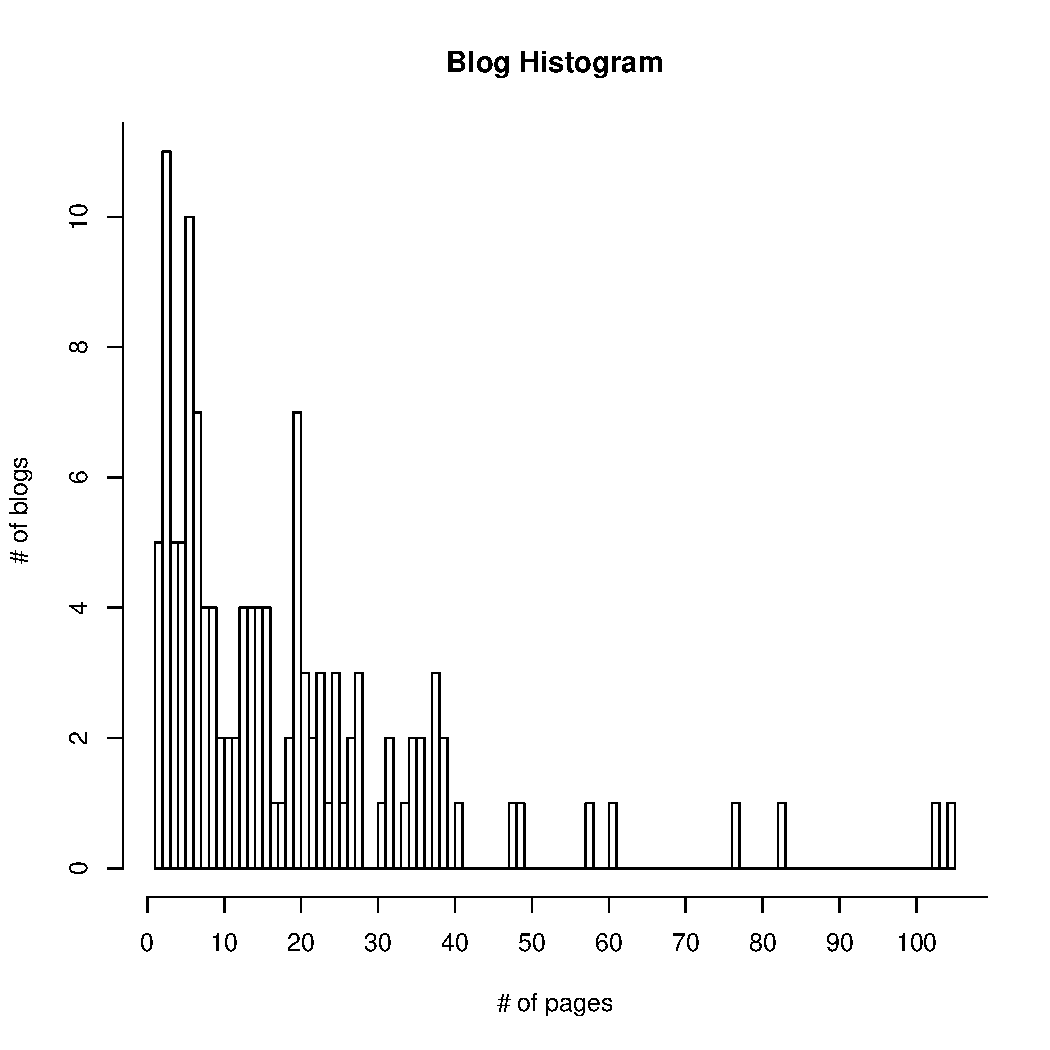
\includegraphics[width=.8\textwidth]{../Rplots.pdf}
\caption{Original partinioning based on data}
\end{figure}

\begin{figure}[H]
\centering 
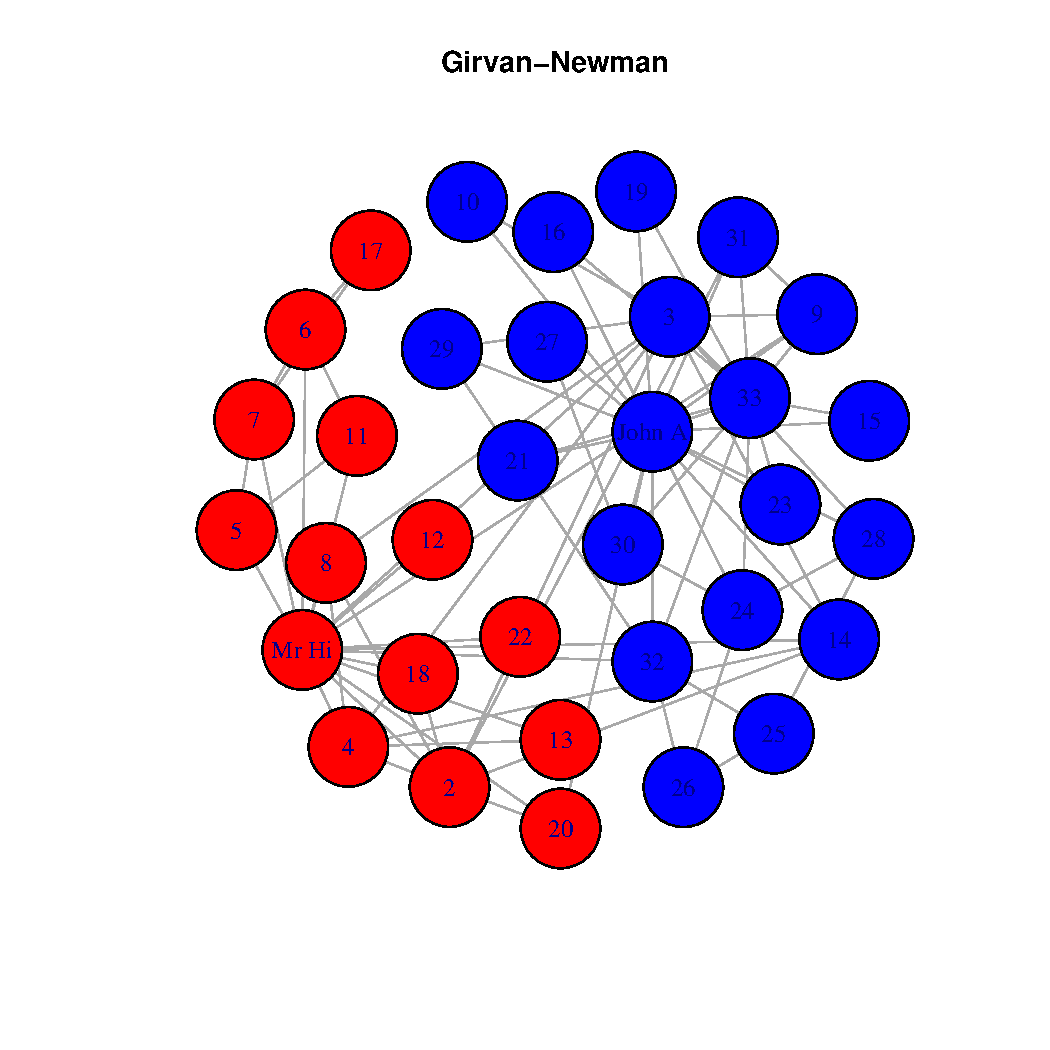
\includegraphics[width=.8\textwidth]{../Rplots1.pdf}
\caption{Predicted partitioning based on Girvan-Newman}
\end{figure}

\begin{figure}[H]
\centering 
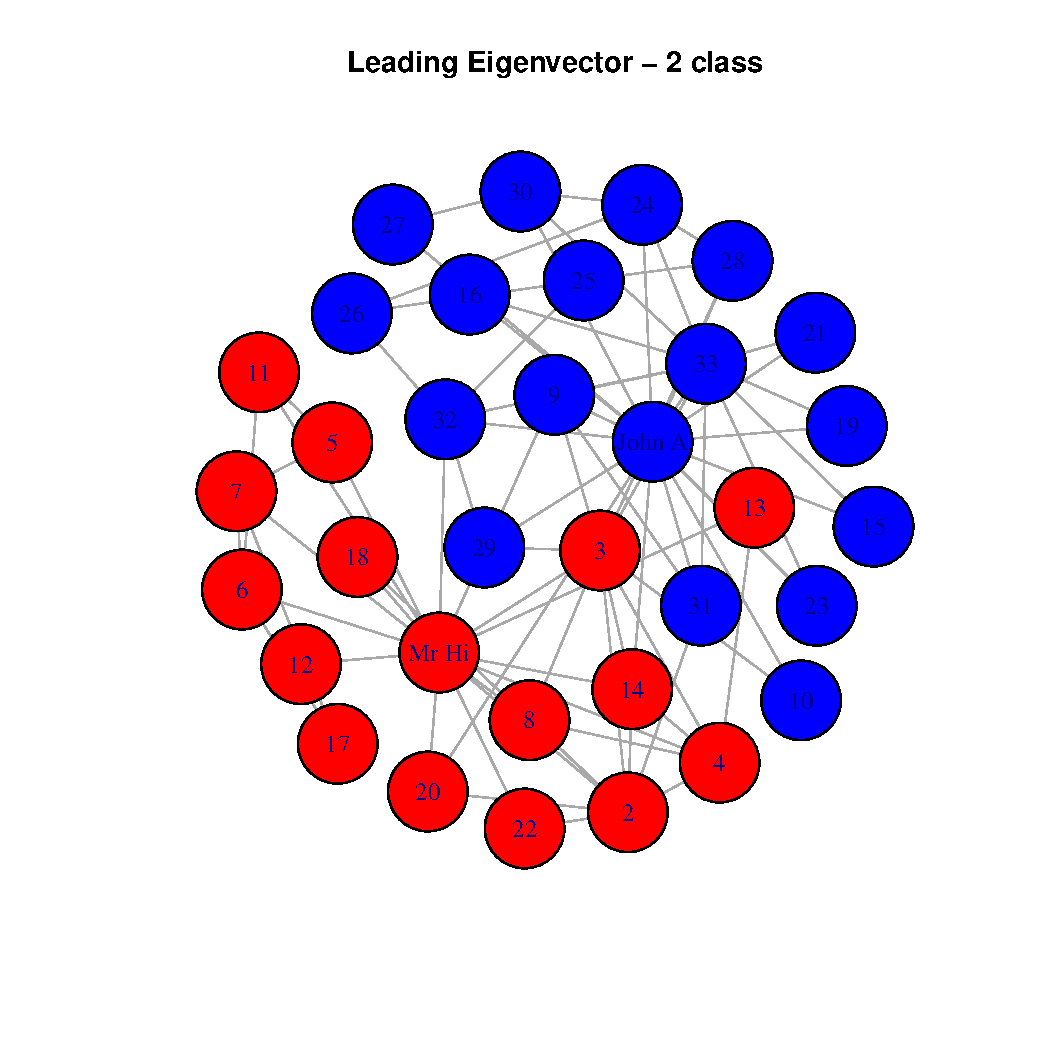
\includegraphics[width=.8\textwidth]{../Rplots2.pdf}
\caption{Predicted partitioning based on Leading Eigenvector Method}
\end{figure}


%
%\lstset{
%    language=R,
%    label=code:q1,
%    caption={R script to do the maths and plot}
%}
%\lstinputlisting{../q1/maths.r}
%%
%\lstset{
%    language=bash,
%    label=code:q1_test,
%    caption={Bash script to extract text from webpage, ignoring links}
%}
%\lstinputlisting{../process.sh}







%\section{Question 2}

\subsection{The Question}

\begin{flushleft}

What 5 movies received the most ratings? Show the movies and
the number of ratings sorted by number of ratings.

\end{flushleft}
\subsection{The Answer}

There review infromation is read in and appeneded to each movie. There is a counter that counter the number of reviews for each movie. This could also be determined by checking the length of the review list for each movie. 


\begin{lstlisting}[caption={Python code for question 2}]

def q2(movies):
	clearScore(movies)
	for i in reviews:
		movies[i.item-1].scores.append(float(i.score))
		movies[i.item-1].cnt +=1

	for i in movies:
		i.avgr();

	# MOST RATING
	mRate = sorted(movies, key=lambda x:x.cnt, reverse=True)
	f = open("q2.txt", "w")
	print "\n\tQ2: Most Ratings"
	for i in range(0,5):
		print  mRate[i].cnt, mRate[i].title
		f.write("% d,  \"%s\"\n" % (mRate[i].cnt, mRate[i].title))
	f.close()

\end{lstlisting}

\begin{flushleft}

\begin{table}[h]
\centering
\setlength{\tabcolsep}{12pt}
\begin{tabular}{|ll|}

\hline
583 & Star Wars (1977)          \\ \hline
509 & Contact (1997)            \\ \hline
508 & Fargo (1996)              \\ \hline
507 & Return of the Jedi (1983) \\ \hline
485 & Liar Liar (1997)         \\ \hline
\end{tabular}
\caption{Movies with Most Ratings}
\end{table}
\end{flushleft}





%\section{Question 2}

\subsection{The Question}

\begin{flushleft}

Create an ASCII and JPEG dendrogram that clusters (i.e., HAC)
the most similar blogs (see slides 12 \& 13).  Include the JPEG in
your report and upload the ascii file to github (it will be too
unwieldy for inclusion in the report).

\end{flushleft}
\subsection{The Answer}

The Python function used to produce the ascii and jpeg dendrograms is provided in the book \cite{PCI}. The output of the script was redirected to a text file ``ascii.txt''. 

\lstset{
    language=Python,
    label=code:q1,
    caption={Python script to produce dendrograms}
}
\lstinputlisting{../q2/q2.py}

\begin{figure}
\centering
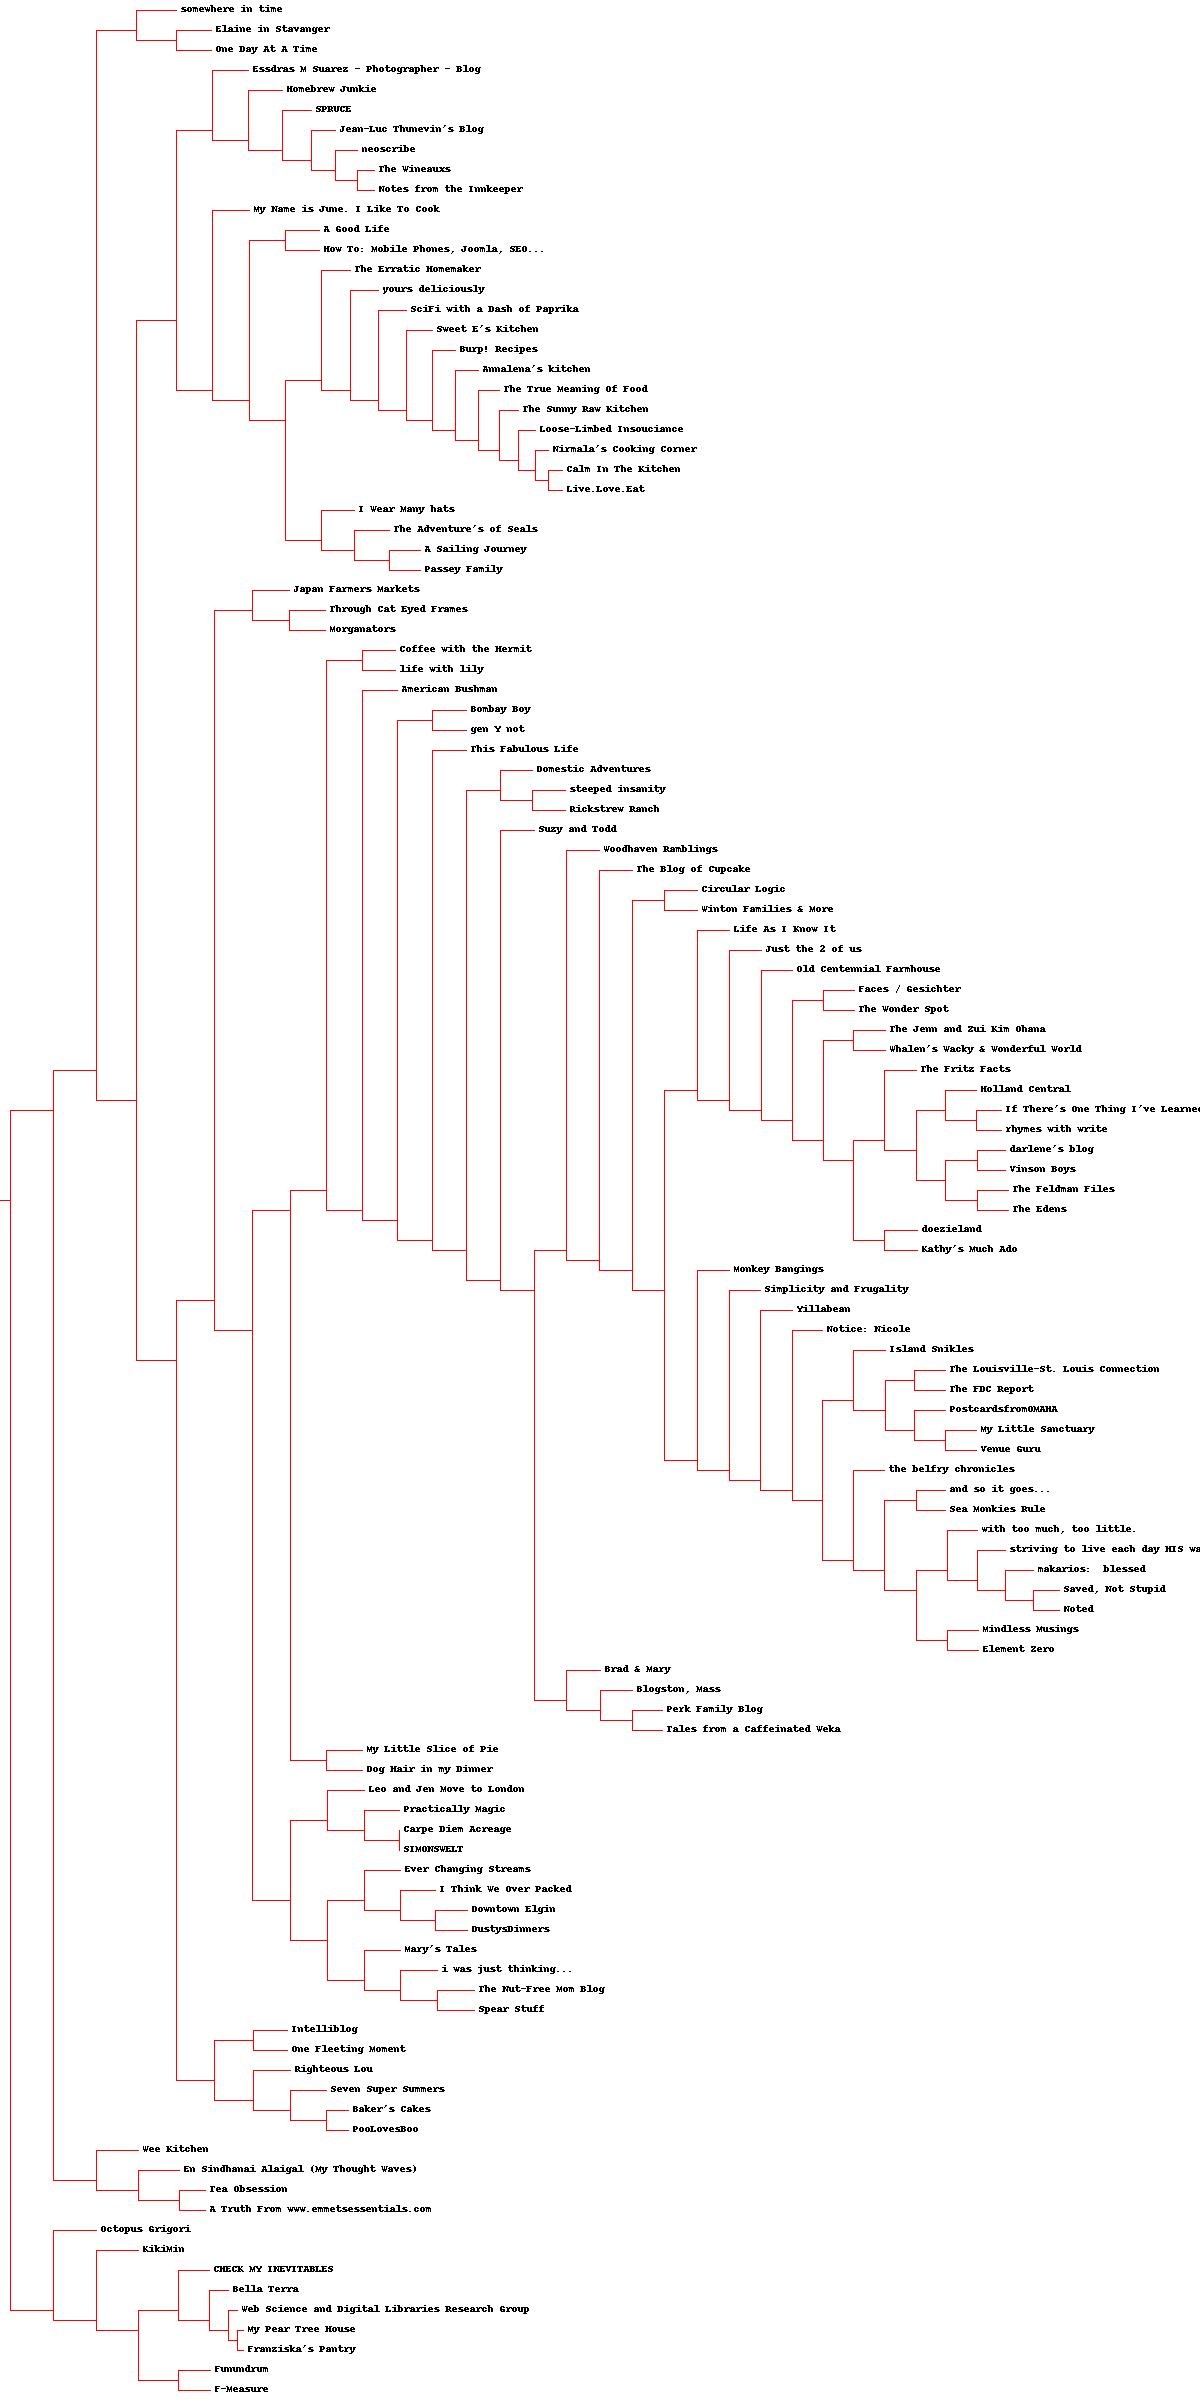
\includegraphics[height=25cm]{../q2/blogdendro.jpg}
\caption{JPEG dendrogram}
\end{figure}








%\section{Question 3}

\subsection{The Question}

\begin{flushleft}

 Cluster the blogs using K-Means, using k=5,10,20. (see slide 18).
How many interations were required for each value of k?

\end{flushleft}
\subsection{The Answer}

The Python function used to produce the K-Means is provided in the book \cite{PCI}. Clustering into 5 clusters required 7 iterations. Clustering into 10 clusters required 6 iterations. Clustering into 20 clusters required 6 iterations.  The terminal output for the script is provided and displays that cluster members


\lstset{
    language=Python,
    label=code:q1,
    caption={Python script to produce dendrograms}
}
\lstinputlisting{../q3/q3.py}


\begin{figure}
\centering
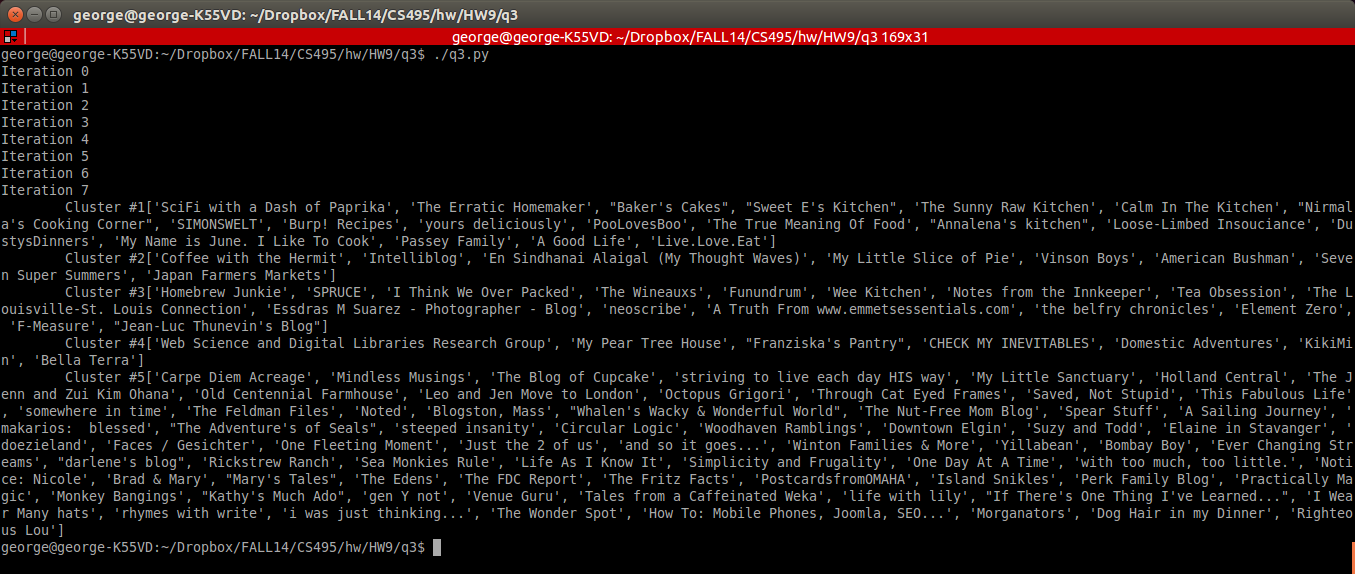
\includegraphics[width=\textwidth]{../q3/clust5.png}
\caption{Terminal output from K-Means CLustering, k = 5}
\end{figure}


\begin{figure}
\centering
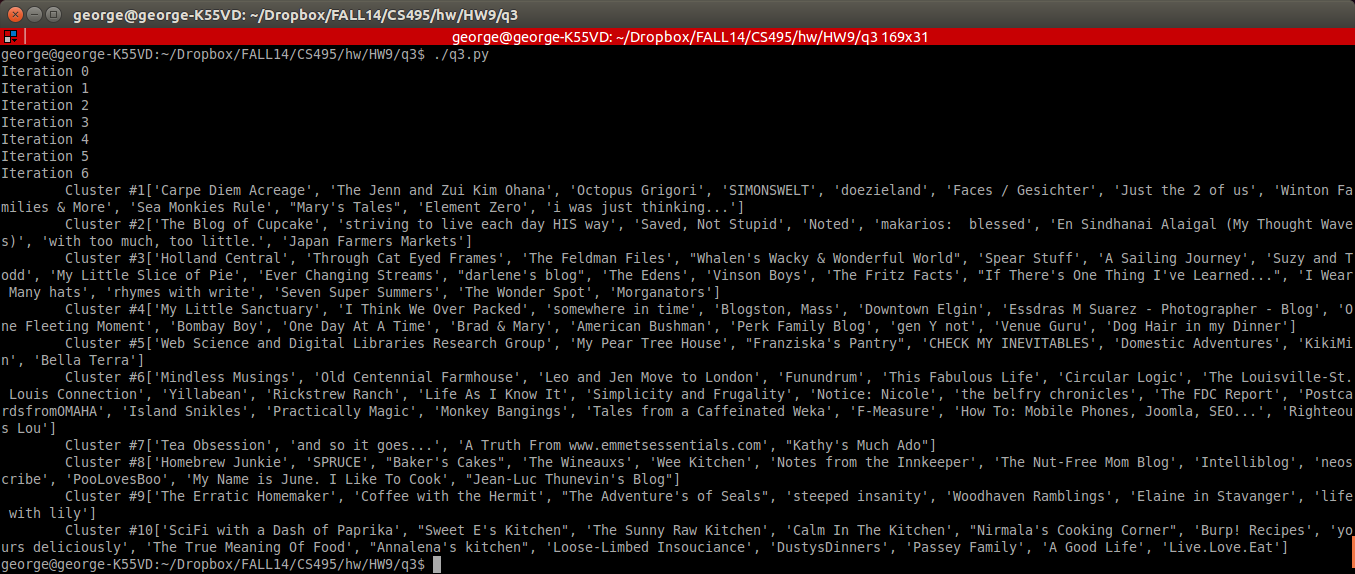
\includegraphics[width=\textwidth]{../q3/clust10.png}
\caption{Terminal output from K-Means CLustering, k = 10}
\end{figure}

\begin{figure}
\centering
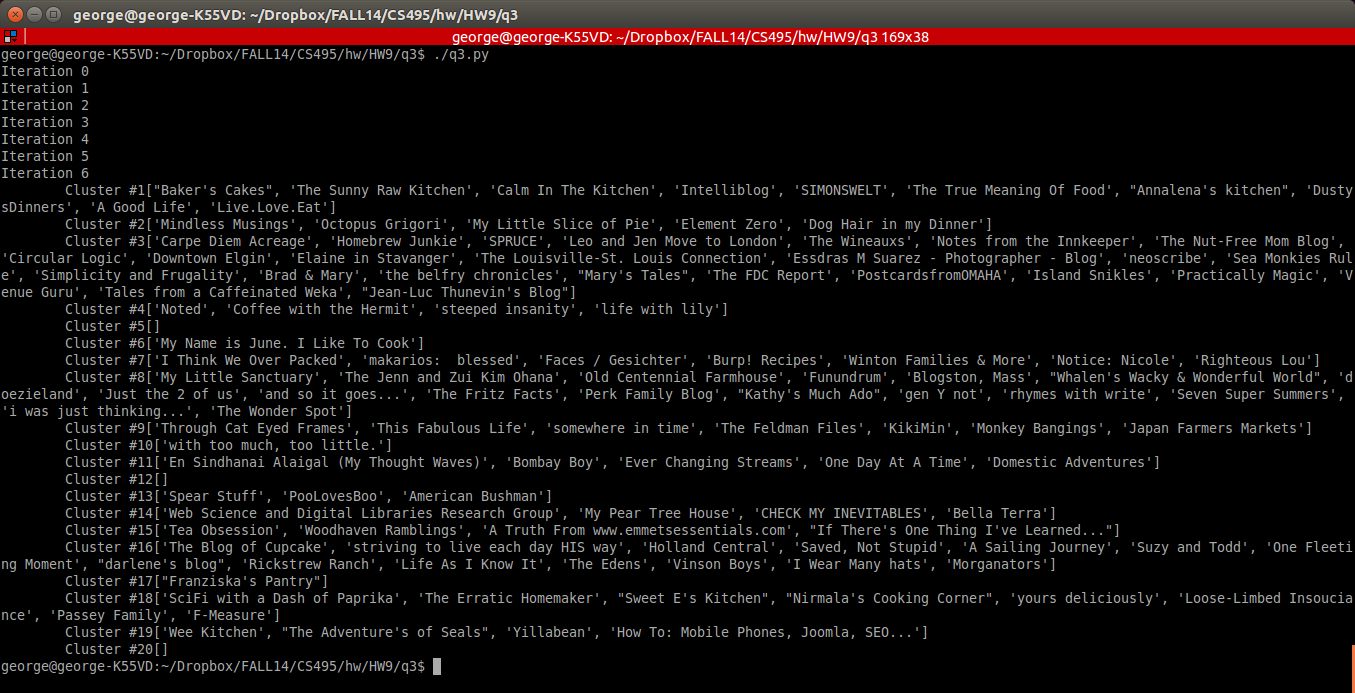
\includegraphics[width=\textwidth]{../q3/clust20.png}
\caption{Terminal output from K-Means CLustering, k = 20}
\end{figure}




%\section{Question 4}

\subsection{The Question}

\begin{flushleft}

 Use MDS to create a JPEG of the blogs similar to slide 29.  
How many iterations were required?

\end{flushleft}
\subsection{The Answer}


The Python function used to produce the MDS plot is provided in the book \cite{PCI}. The algorithm required 353 iterations to converge. The terminal output it attached.

\lstset{
    language=Python,
    label=code:q1,
    caption={Python script to produce dendrograms}
}
\lstinputlisting{../q4/q4.py}


\begin{figure}
\centering
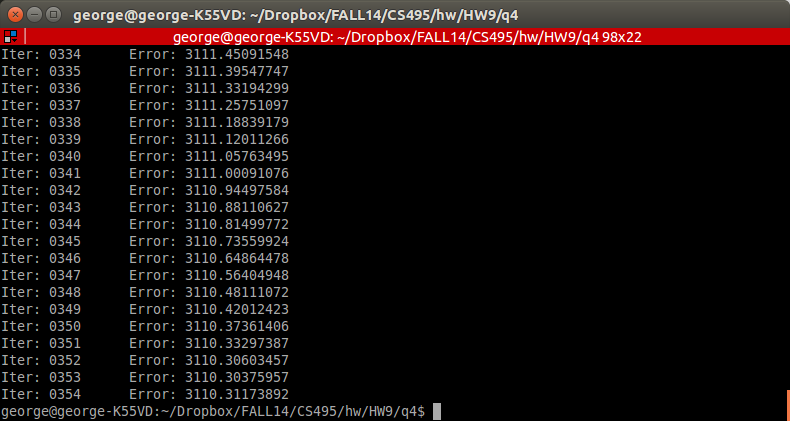
\includegraphics[width=\textwidth]{../q4/mds.png}
\caption{Terminal output from Multi-Dimensional Scaling}
\end{figure}

\begin{figure}
\centering
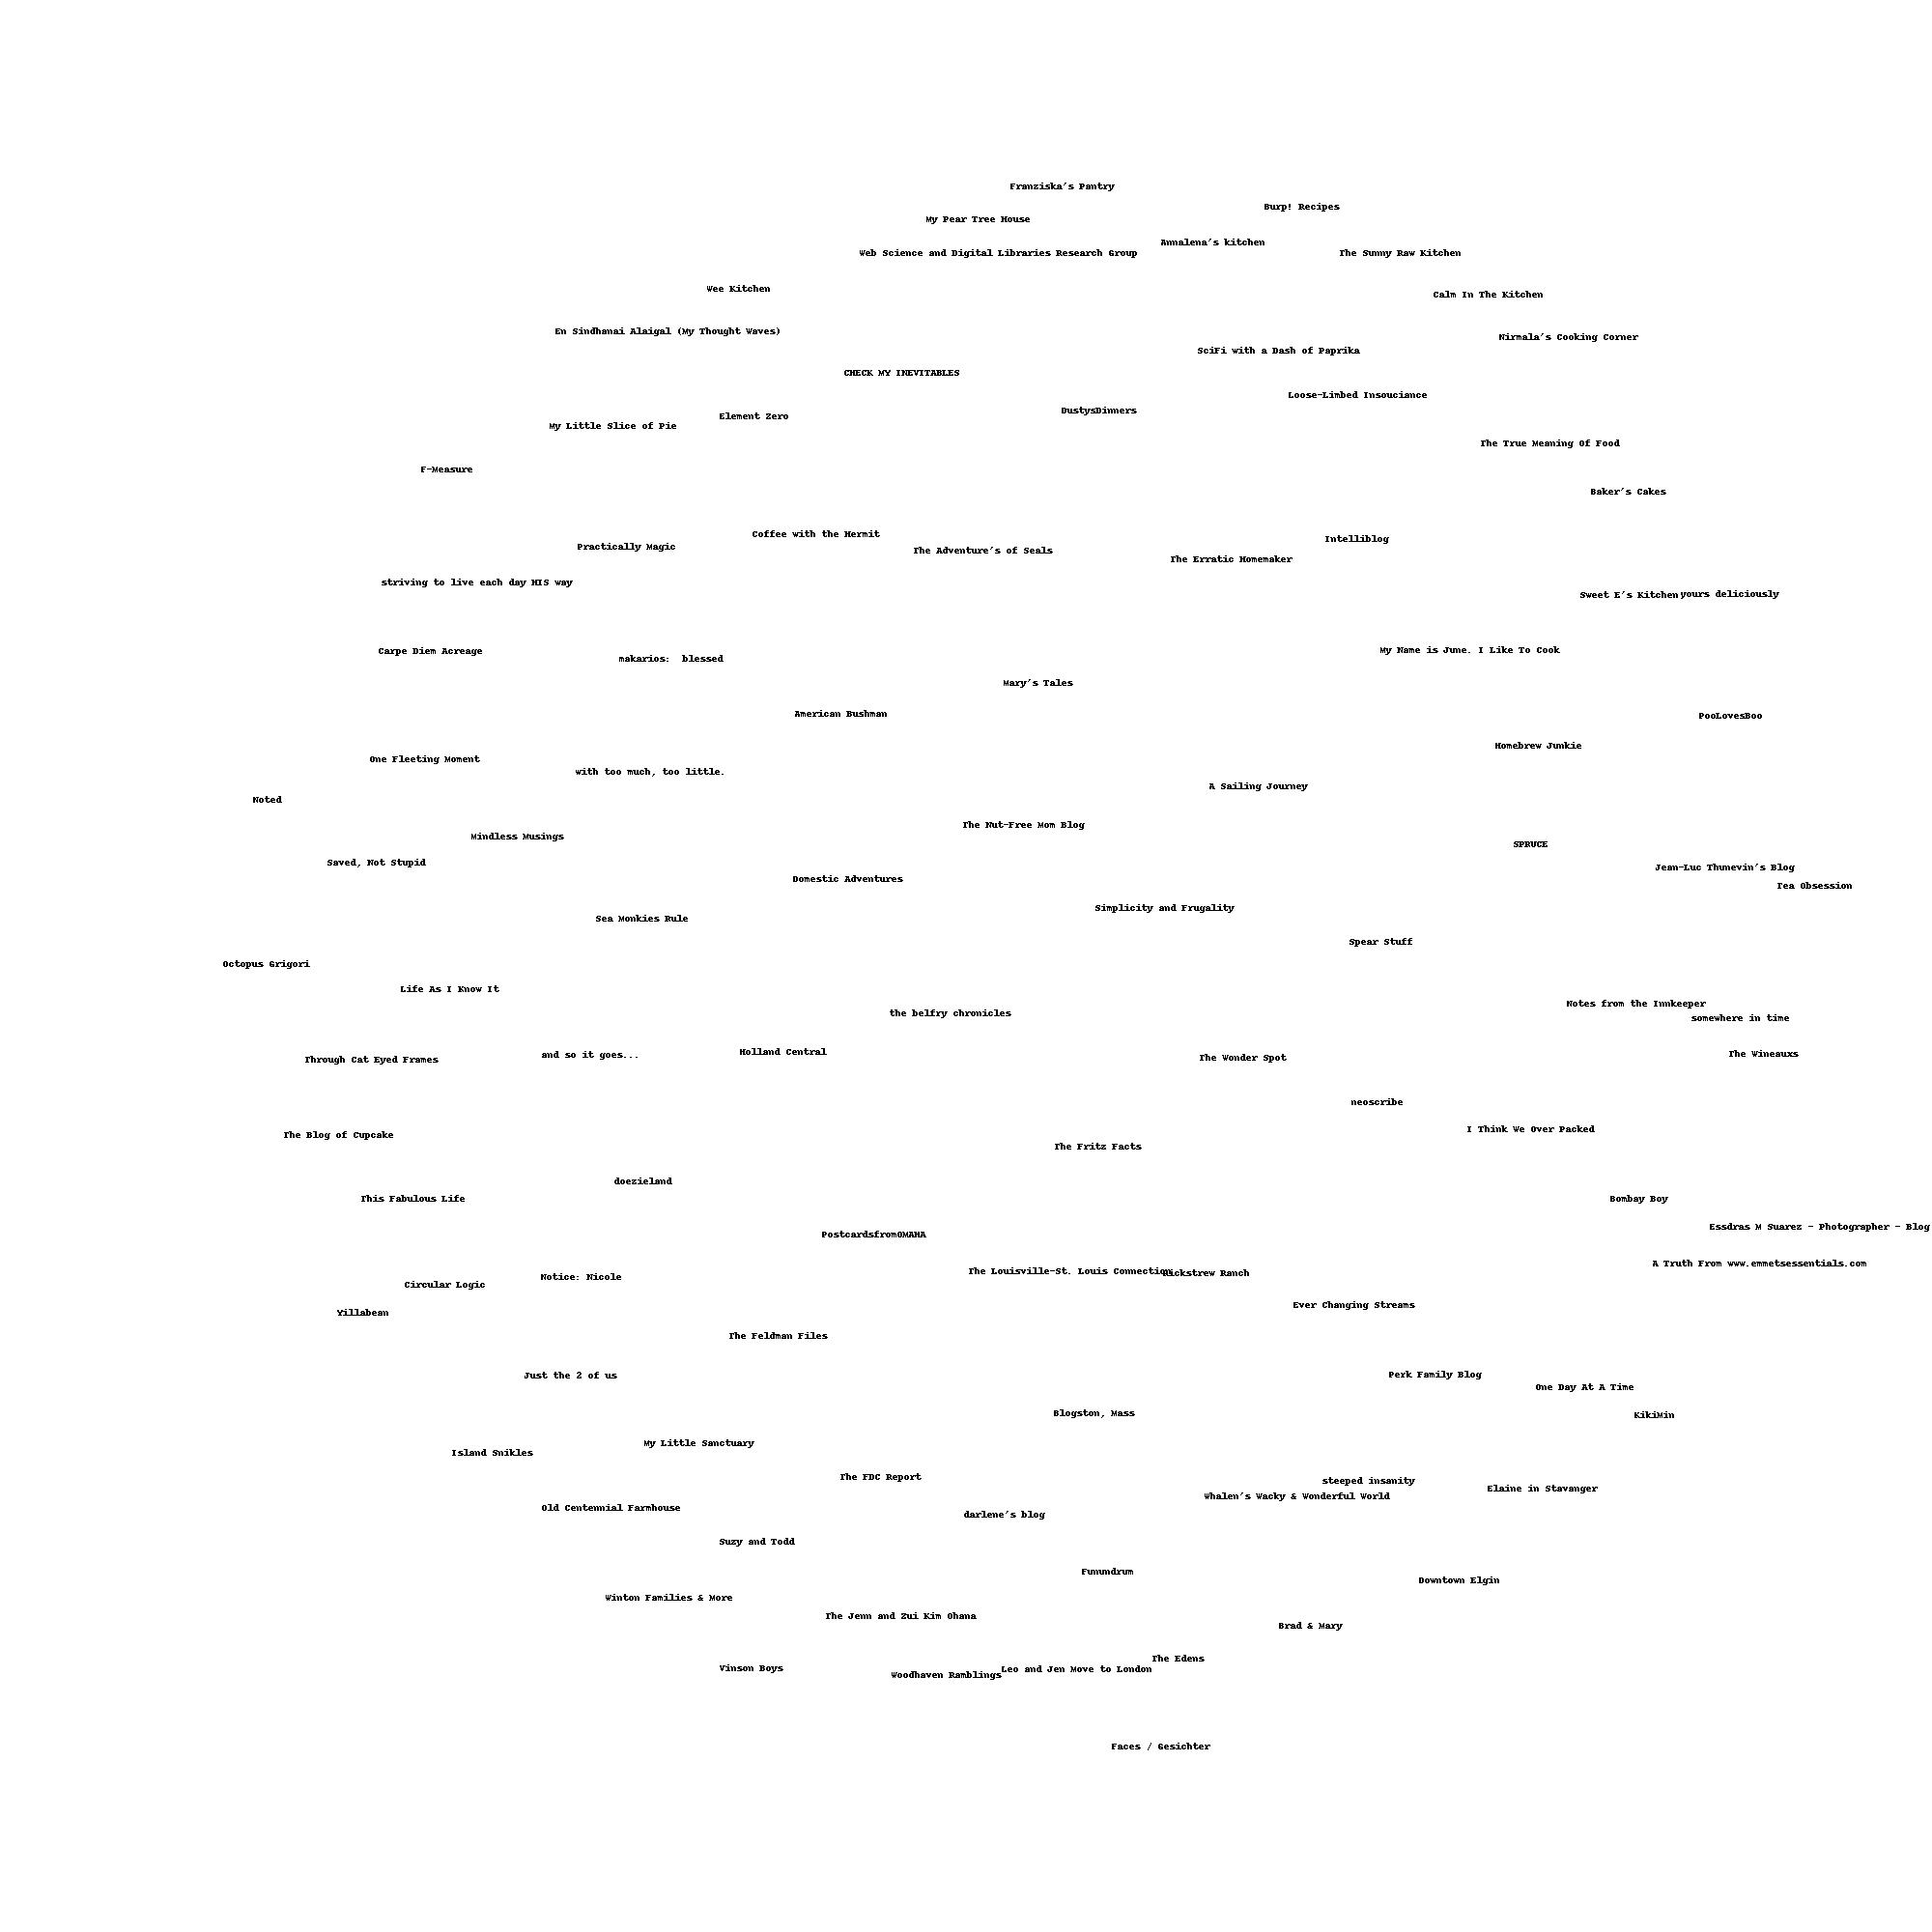
\includegraphics[width=\textwidth]{../q4/blogs2d}
\caption{Multi-Dimensional Scaling of the blogs}
\end{figure}





%\section{Question 6}

\subsection{The Question}

\begin{flushleft}

Which 5 raters rated the most films? Show the raters' IDs and
the number of films each rated.

\end{flushleft}
\subsection{The Answer}

The reviews were read line by line and appened to each user. The users were then sorted based on number of reviews. The top five were taken from the sorted list. 


\begin{lstlisting}[caption={Python code for question 6}]
def q6(users):
	for i in reviews:
		users[i.user-1].cnt += 1

	usr = sorted(users,key=lambda x:x.cnt, reverse=True)

	# 
	f = open("q6.txt", "w")
	print "\n\tQ6: Rated most pics"
	print  "cnt, id"
	for i in range(0,5):
		print  usr[i].cnt, usr[i].id
		f.write("%d,  %d\n" % (usr[i].cnt, usr[i].id))
	f.close()
\end{lstlisting}


\begin{flushleft}


\begin{table}[h]
\setlength{\tabcolsep}{12pt}
\centering
\begin{tabular}{|ll|}
\hline
737 & 405 \\ \hline
685 & 655 \\ \hline
636 & 13  \\ \hline
540 & 450 \\ \hline
518 & 276 \\ \hline
\end{tabular}
\caption{Raters with the Most Reviews}
\end{table}


\end{flushleft}





%%%%%%%%%%%%%%%%%%%%%%%%%%%%%%%%%%%%%%%%%%%%%%%%%%%%%%%%%%%


%%%%%%%%%%%%%%%%%%%%%%%%%%%%%%%%%%%%%%%%%%%%%%%%%%%%%%%%%%%
\nocite{*}
\bibliography{sources}
\bibliographystyle{unsrt}




%%%%%%%%%%%%%%%%%%%%%%%%%%%%%%%%%%%%%%%%%%%%%%%%%%%%%%%%%%%

%%%%%%%%%%%%%%%%%%%%%%%%%%%%%%%%%%%%%%%%%%%%%%%%%%%%%%%%%%%



%%%%%%%%%%%%%%%%%%%%%%%%%%%%%%%%%%%%%%%%%%%%%%%%%%%%%%%%%%%




%%%%%%%%%%%%%%%%%%%%%%%%%%%%%%%%%%%%%%%%%%%%%%%%%%%%%%%%%%%



%%%%%%%%%%%%%%%%%%%%%%%%%%%%%%%%%%%%%%%%%%%%%%%%%%%%%%%%%%%




\end{document}


